\chapter{Électronégativité, polarité et interactions entre molécules}\label{ch:g11:polarity-and-cohesion}

Un gecko court sur une vitre et reste suspendu au verre par un seul
doigt, sans colle ni ventouse. Une \omterm{def:g7:atoms-and-molecules:molecule}{molécule} d'eau, \ce{H2O}, est plus
légère qu'une \omterm{def:g7:atoms-and-molecules:molecule}{molécule} de sulfure d'hydrogène, \ce{H2S}, et pourtant
l'eau bout à \qty{100}{\celsius} alors que le sulfure d'hydrogène reste
gazeux jusqu'à \qty{-60}{\celsius}. Les deux histoires parlent de la
même chose~: les forces qui retiennent les \omterm{def:g7:atoms-and-molecules:molecule}{molécules} les unes aux autres,
et à d'autres objets. Elles sont bien plus faibles que les \omterm{def:g10:lewis-and-shape:covalent-bond}{liaisons
covalentes} à l'intérieur d'une \omterm{def:g7:atoms-and-molecules:molecule}{molécule}, mais elles décident si une
substance est gazeuse, liquide ou solide à température ambiante, et si
un gecko tombe.

\begin{recall}
Une \omterm{def:g10:lewis-and-shape:covalent-bond}{liaison covalente} est un doublet d'\omterm{def:g9:inside-the-atom:nucleus}{électrons} mis en commun par deux
\omterm{def:g7:atoms-and-molecules:atom}{atomes}~; les \omterm{def:g10:lewis-and-shape:lewis-structure}{schémas de Lewis} montrent les \omterm{def:g10:lewis-and-shape:lone-pair}{doublets liants} et non
liants, et les doublets autour d'un \omterm{def:g7:atoms-and-molecules:atom}{atome} central décident de la
géométrie d'une \omterm{def:g7:atoms-and-molecules:molecule}{molécule} (\cref{ch:g10:lewis-and-shape}). Les \omterm{def:g9:ions:ion}{ions}
portent une charge~; dans un solide ionique, les \omterm{def:g9:ions:ion}{ions} positifs et
négatifs s'attirent (\cref{ch:g9:ions}).
\end{recall}

\begin{omfigure}
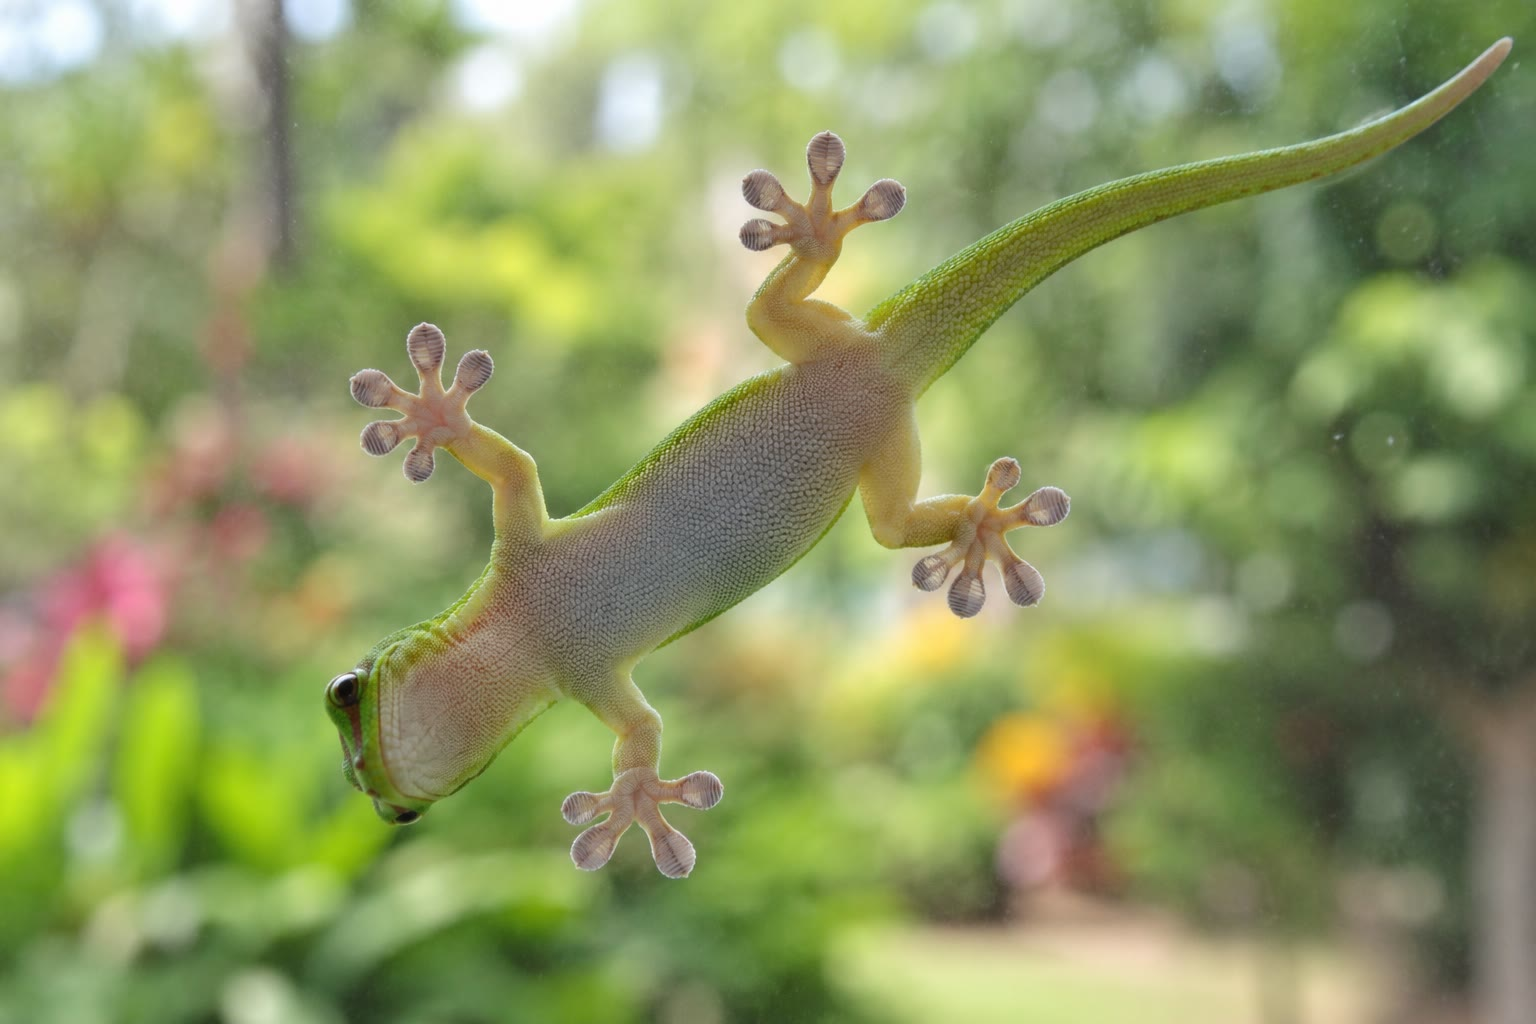
\includegraphics[width=0.5\linewidth]{images/book1/ai/g11-gecko-glass.jpg}

{\small Un gecko sur une vitre~: les coussinets de ses doigts tiennent
grâce à des forces entre \omterm{def:g7:atoms-and-molecules:molecule}{molécules}.}
\end{omfigure}

\section{L'électronégativité}

\begin{definition}[Électronégativité]\label{def:g11:polarity-and-cohesion:electronegativity}
L'\emph{électronégativité}\index{electronegativite@électronégativité} d'un élément mesure
la force avec laquelle ses \omterm{def:g7:atoms-and-molecules:atom}{atomes}, dans une \omterm{def:g7:atoms-and-molecules:molecule}{molécule}, attirent les
\omterm{def:g9:inside-the-atom:nucleus}{électrons} des liaisons qu'ils partagent. C'est un nombre sans unité~;
sur l'échelle usuelle, elle va d'environ 0.8 à environ 4.
\end{definition}

\begin{omfigure}
% ledger: en:H, en:Li, en:Be, en:B, en:C, en:N, en:O, en:F, en:Na, en:Mg, en:Al, en:Si, en:P, en:S, en:Cl, en:K, en:Ca
\omperiodictable[upto=20, f block=false, cell=0.9cm, values={H/2.20,
  Li/0.98, Be/1.57, B/2.04, C/2.55, N/3.04, O/3.44, F/3.98, Na/0.93,
  Mg/1.31, Al/1.61, Si/1.90, P/2.19, S/2.58, Cl/3.16, K/0.82, Ca/1.00},
  highlight={F,O,N,Cl}]

{\small \omterm{def:g11:polarity-and-cohesion:electronegativity}{Électronégativités} des vingt premiers éléments (échelle de
Pauling~; aucune n'est donnée pour l'hélium, le néon et l'argon, qui ne
forment pas de liaisons ici). En surbrillance~: les quatre éléments les
plus électronégatifs.}
\end{omfigure}

\begin{proposition}[Les tendances dans le tableau]\label{prop:g11:polarity-and-cohesion:trends}
% ledger: en:F, en:Li, en:Cl, en:K
L'\omterm{def:g11:polarity-and-cohesion:electronegativity}{électronégativité} augmente de gauche à droite le long d'une \omterm{def:g9:periodic-table-first-look:period}{période}
et diminue de haut en bas dans un groupe. Le fluor (3.98) est l'élément
le plus électronégatif~; les \omterm{def:g10:electron-shells:family}{métaux alcalins} sont les moins
électronégatifs (lithium 0.98, potassium 0.82).
\end{proposition}

\begin{proof}
Lecture du tableau~: le long de la \omterm{def:g9:periodic-table-first-look:period}{période} 2, $0.98 < 1.57 < 2.04 < 2.55 < 3.04 <
3.44 < 3.98$~; dans le \omterm{def:g9:periodic-table-first-look:period}{groupe} 17, le fluor ($3.98$) est au-dessus du
chlore ($3.16$)~; dans le \omterm{def:g9:periodic-table-first-look:period}{groupe} 1, $2.20$, $0.98$, $0.93$, $0.82$.
(La raison en est expliquée dans le volume de première année
d'université.)
\end{proof}

\begin{history}[L'échelle de Pauling, 1932]
Le chimiste Linus Pauling construisit la première échelle
d'\omterm{def:g11:polarity-and-cohesion:electronegativity}{électronégativité} en 1932, à partir des énergies de liaison entre
\omterm{def:g7:atoms-and-molecules:atom}{atomes} différents. Il donna au fluor la plus grande valeur, et l'échelle
utilisée dans ce chapitre porte encore son nom.
\end{history}

\section{Liaisons polarisées et molécules polaires}

\begin{definition}[Liaison polarisée, charge partielle]\label{def:g11:polarity-and-cohesion:polar-bond}
Une \omterm{def:g10:lewis-and-shape:covalent-bond}{liaison covalente} entre deux \omterm{def:g7:atoms-and-molecules:atom}{atomes} d'\omterm{def:g11:polarity-and-cohesion:electronegativity}{électronégativités} différentes
est une \emph{liaison polarisée}\index{liaison polarisee@liaison polarisée}~: le doublet
partagé se trouve plus près de l'\omterm{def:g7:atoms-and-molecules:atom}{atome} le plus électronégatif. Cet \omterm{def:g7:atoms-and-molecules:atom}{atome}
porte une petite \emph{charge partielle}\index{charge partielle}
négative, notée $\delta^-$, et l'autre \omterm{def:g7:atoms-and-molecules:atom}{atome} une charge partielle
positive égale, $\delta^+$.
\end{definition}

\begin{proposition}[Quand une liaison est-elle polarisée~?]\label{prop:g11:polarity-and-cohesion:polar-bond}
% ledger: en:C, en:H, en:O, en:Na, en:Cl
Une liaison entre deux \omterm{def:g7:atoms-and-molecules:atom}{atomes} identiques n'est pas polarisée. Entre
\omterm{def:g7:atoms-and-molecules:atom}{atomes} différents, plus la différence d'\omterm{def:g11:polarity-and-cohesion:electronegativity}{électronégativité} est grande,
plus la liaison est polarisée~; en règle pratique, une différence
inférieure à 0.4 environ (comme pour \ce{C-H}, $2.55 - 2.20 = 0.35$) est
considérée comme non polarisée. Quand la différence est très grande
(comme pour Na et Cl, $3.16 - 0.93 = 2.23$), les \omterm{def:g9:inside-the-atom:nucleus}{électrons} ne sont pas
mis en commun mais transférés~: le composé est ionique.
\end{proposition}

\begin{proof}
Admis~: cela découle de la définition de l'\omterm{def:g11:polarity-and-cohesion:electronegativity}{électronégativité}, les seuils
étant des conventions.
\end{proof}

\begin{definition}[Molécules polaires et apolaires]\label{def:g11:polarity-and-cohesion:polar-molecule}
Une \omterm{def:g7:atoms-and-molecules:molecule}{molécule} est une \emph{molécule polaire}\index{molecule polaire@molécule polaire} si
le centre de ses \omterm{def:g11:polarity-and-cohesion:polar-bond}{charges partielles} positives et le centre de ses
\omterm{def:g11:polarity-and-cohesion:polar-bond}{charges partielles} négatives ne coïncident pas~; s'ils coïncident, c'est
une \emph{molécule apolaire}\index{molecule apolaire@molécule apolaire}.
\end{definition}

\begin{method}[Une molécule est-elle polaire~?]\label{met:g11:polarity-and-cohesion:polar}
\begin{enumerate}
  \item Établir le \omterm{def:g10:lewis-and-shape:lewis-structure}{schéma de Lewis} et déterminer la géométrie de la
        \omterm{def:g7:atoms-and-molecules:molecule}{molécule}.
  \item Repérer les \omterm{def:g11:polarity-and-cohesion:polar-bond}{liaisons polarisées} par $\delta^+$ et $\delta^-$.
  \item S'il n'y a aucune \omterm{def:g11:polarity-and-cohesion:polar-bond}{liaison polarisée}, la \omterm{def:g7:atoms-and-molecules:molecule}{molécule} est apolaire.
        Sinon, examiner la géométrie~: si les \omterm{def:g11:polarity-and-cohesion:polar-bond}{liaisons polarisées} sont
        disposées symétriquement autour du centre, leurs effets se
        compensent et la \omterm{def:g7:atoms-and-molecules:molecule}{molécule} est apolaire~; sinon, elle est polaire.
\end{enumerate}
\end{method}

\begin{omfigure}
\begin{tikzpicture}[font=\small]
  % water
  \begin{scope}
    \node[aO] (o) at (0,0) {};
    \node[aH] (h1) at (-0.82,-0.6) {};
    \node[aH] (h2) at (0.82,-0.6) {};
    \begin{scope}[on background layer]
      \draw[bond] (o.center) -- (h1.center); \draw[bond] (o.center) -- (h2.center);
    \end{scope}
    \node[omThm] at (0,0.55) {$2\delta^-$};
    \node[omDef] at (-1.22,-0.5) {$\delta^+$};
    \node[omDef] at (1.22,-0.5) {$\delta^+$};
    \fill[omDef] (0,-0.6) circle (0.06);
    \fill[omThm] (0,0) circle (0.06);
    \draw[densely dotted, black!60] (-0.82,-0.6) -- (0.82,-0.6);
    \draw[<-, black!60] (0.08,-0.64) -- (1.55,-1.05) node[right, align=left,
      font=\footnotesize] {centre des\\ $\delta^+$};
    \node[align=center, anchor=north] at (0,-1.8) {eau~: coudée, \textbf{polaire}};
  \end{scope}
  % carbon dioxide
  \begin{scope}[xshift=6cm]
    \node[aO] (o1) at (-1.15,0) {};
    \node[aC] (c) at (0,0) {};
    \node[aO] (o2) at (1.15,0) {};
    \begin{scope}[on background layer]
      \draw[bond, double, double distance=1.6pt] (o1.center) -- (c.center);
      \draw[bond, double, double distance=1.6pt] (c.center) -- (o2.center);
    \end{scope}
    \node[omThm] at (-1.15,0.55) {$\delta^-$};
    \node[omThm] at (1.15,0.55) {$\delta^-$};
    \node[omDef] at (0,0.55) {$2\delta^+$};
    \draw[->, omProp, thick] (-0.25,-0.45) -- (-1.0,-0.45);
    \draw[->, omProp, thick] (0.25,-0.45) -- (1.0,-0.45);
    \node[align=center, anchor=north] at (0,-1.8) {dioxyde de carbone~: linéaire,\\
      \textbf{apolaire}};
  \end{scope}
\end{tikzpicture}

{\small Dans l'eau, la forme coudée place le centre des \omterm{def:g11:polarity-and-cohesion:polar-bond}{charges
partielles} positives (entre les \omterm{def:g7:atoms-and-molecules:atom}{atomes} d'hydrogène) au-dessous de
l'\omterm{def:g7:atoms-and-molecules:atom}{atome} d'oxygène~: la \omterm{def:g7:atoms-and-molecules:molecule}{molécule} est polaire. Dans le dioxyde de carbone,
les deux \omterm{def:g11:polarity-and-cohesion:polar-bond}{liaisons polarisées} tirent dans des sens opposés (flèches) et
se compensent~: les centres des charges coïncident sur l'\omterm{def:g7:atoms-and-molecules:atom}{atome} de
carbone.}
\end{omfigure}


\begin{example}[Quatre molécules]\label{ex:g11:polarity-and-cohesion:four}
Le chlorure d'hydrogène \ce{HCl} a une \omterm{def:g11:polarity-and-cohesion:polar-bond}{liaison polarisée} et il est
polaire, le chlore portant $\delta^-$. L'ammoniac \ce{NH3}, une pyramide
de trois \omterm{def:g11:polarity-and-cohesion:polar-bond}{liaisons polarisées} \ce{N-H}, est polaire, l'azote portant
$\delta^-$. Le méthane \ce{CH4} n'a que des liaisons \ce{C-H} presque
non polarisées~: il est apolaire. Le tétrachlorométhane \ce{CCl4} a
quatre \omterm{def:g11:polarity-and-cohesion:polar-bond}{liaisons polarisées} \ce{C-Cl}, mais placées aux sommets d'un
tétraèdre régulier~: leurs effets se compensent et la \omterm{def:g7:atoms-and-molecules:molecule}{molécule} est
apolaire.
\end{example}

\section{Les interactions de van der Waals}

\begin{definition}[Interaction de van der Waals]\label{def:g11:polarity-and-cohesion:van-der-waals}
Une \emph{interaction de van der Waals}\index{interaction de van der Waals}
est une faible attraction entre \omterm{def:g7:atoms-and-molecules:molecule}{molécules} voisines, qui existe entre
toutes les \omterm{def:g7:atoms-and-molecules:molecule}{molécules}, polaires ou non~: les \omterm{def:g9:inside-the-atom:nucleus}{électrons} de chaque \omterm{def:g7:atoms-and-molecules:molecule}{molécule}
sont sans cesse en mouvement, et les charges inégalement réparties d'un
instant dans une \omterm{def:g7:atoms-and-molecules:molecule}{molécule} attirent celles de ses voisines. Entre
\omterm{def:g11:polarity-and-cohesion:polar-molecule}{molécules polaires}, les \omterm{def:g11:polarity-and-cohesion:polar-bond}{charges partielles} permanentes ajoutent une
attraction supplémentaire.
\end{definition}


\begin{proposition}[Les grosses molécules s'attirent davantage]\label{prop:g11:polarity-and-cohesion:size}
Les \omterm{def:g11:polarity-and-cohesion:van-der-waals}{interactions de van der Waals} croissent avec la taille des
\omterm{def:g7:atoms-and-molecules:molecule}{molécules}, c'est-à-dire avec leur nombre d'\omterm{def:g9:inside-the-atom:nucleus}{électrons}~; entre \omterm{def:g7:atoms-and-molecules:molecule}{molécules}
semblables, les plus grosses ont les températures de fusion et
d'ébullition les plus élevées.
\end{proposition}

\begin{proof}
Admis~: un nuage électronique plus grand se déforme plus facilement, si
bien que ses charges instantanées sont plus grandes, et il a davantage
de contact avec ses voisins.
\end{proof}

\begin{example}[Les halogènes]\label{ex:g11:polarity-and-cohesion:halogens}
% ledger: bp:F2, bp:Cl2, bp:Br2, bp:I2 (K values converted)
Les \omterm{def:g7:atoms-and-molecules:molecule}{molécules} \ce{F2}, \ce{Cl2}, \ce{Br2}, \ce{I2} sont toutes apolaires
et de plus en plus grosses. Leurs températures d'ébullition augmentent
avec elles~: \qty{-188}{\celsius}, \qty{-34}{\celsius}, \qty{59}{\celsius}
et \qty{184}{\celsius}. À température ambiante, le difluor et le dichlore
sont des gaz, le dibrome un liquide, le diiode un solide.
\end{example}

\begin{remark}[Le gecko]\label{rem:g11:polarity-and-cohesion:gecko}
Une seule \omterm{def:g11:polarity-and-cohesion:van-der-waals}{interaction de van der Waals} est minuscule, mais elles
s'additionnent. Les coussinets des doigts d'un gecko sont couverts d'un
tapis dense de poils microscopiques, chacun divisé en pointes encore
plus fines, qui s'approchent assez du verre pour que les \omterm{def:g11:polarity-and-cohesion:van-der-waals}{interactions de
van der Waals} agissent sur une très grande surface totale.
\end{remark}

\section{Les liaisons hydrogène}

\begin{definition}[Liaison hydrogène]\label{def:g11:polarity-and-cohesion:hydrogen-bond}
Une \emph{liaison hydrogène}\index{liaison hydrogene@liaison hydrogène} est une attraction
entre un \omterm{def:g7:atoms-and-molecules:atom}{atome} d'hydrogène lié à un \omterm{def:g7:atoms-and-molecules:atom}{atome} très électronégatif (azote,
oxygène ou fluor), qui porte un $\delta^+$ marqué, et un \omterm{def:g10:lewis-and-shape:lone-pair}{doublet non
liant} d'un autre \omterm{def:g7:atoms-and-molecules:atom}{atome} d'azote, d'oxygène ou de fluor, souvent situé sur
une \omterm{def:g7:atoms-and-molecules:molecule}{molécule} voisine. On la représente par un trait en pointillés, et
les trois \omterm{def:g7:atoms-and-molecules:atom}{atomes} concernés sont presque alignés.
\end{definition}

\begin{omfigure}
\begin{tikzpicture}[font=\small]
  % central water molecule and four neighbours, H-bonds dashed
  \newcommand{\water}[4]{% name, x, y, rotation
    \begin{scope}[shift={(#2,#3)}, rotate=#4]
      \node[aO] (#1o) at (0,0) {};
      \node[aH] (#1a) at (-0.6,-0.45) {};
      \node[aH] (#1b) at (0.6,-0.45) {};
    \end{scope}
    \begin{scope}[on background layer]
      \draw[bond] (#1o.center) -- (#1a.center); \draw[bond] (#1o.center) -- (#1b.center);
    \end{scope}}
  \water{m}{0}{0}{0}
  \water{p}{-1.62}{-1.215}{0}
  \water{q}{1.62}{-1.215}{0}
  \water{r}{-1.435}{1.435}{-8.13}
  \water{s}{1.435}{1.435}{8.13}
  % H-bonds: m's H to p's O and q's O; r's and s's H to m's O
  \draw[dashed, omDef, thick] (ma) -- (po);
  \draw[dashed, omDef, thick] (mb) -- (qo);
  \draw[dashed, omDef, thick] (rb) -- (mo);
  \draw[dashed, omDef, thick] (sa) -- (mo);
\end{tikzpicture}

{\small Les \omterm{def:g11:polarity-and-cohesion:hydrogen-bond}{liaisons hydrogène} (en pointillés) autour d'une \omterm{def:g7:atoms-and-molecules:molecule}{molécule}
d'eau dans l'eau liquide~: ses deux \omterm{def:g7:atoms-and-molecules:atom}{atomes} d'hydrogène se lient aux
\omterm{def:g7:atoms-and-molecules:atom}{atomes} d'oxygène de deux voisines, et les deux \omterm{def:g10:lewis-and-shape:lone-pair}{doublets non liants} de
son \omterm{def:g7:atoms-and-molecules:atom}{atome} d'oxygène reçoivent les \omterm{def:g7:atoms-and-molecules:atom}{atomes} d'hydrogène de deux autres.}
\end{omfigure}


\begin{example}[L'éthanol et le propane]\label{ex:g11:polarity-and-cohesion:ethanol}
% ledger: bp:C2H5OH, bp:C3H8 (K values converted)
L'éthanol, \ce{CH3-CH2-OH} (\qty{46.0}{g/mol}), et le propane,
\ce{CH3-CH2-CH3} (\qty{44.0}{g/mol}), ont des \omterm{def:g7:atoms-and-molecules:molecule}{molécules} de tailles
presque égales. Pourtant, l'éthanol bout à \qty{78}{\celsius} et le
propane à \qty{-42}{\celsius}. Les \omterm{def:g7:atoms-and-molecules:molecule}{molécules} d'éthanol, avec leur groupe
\ce{O-H}, forment entre elles des \omterm{def:g11:polarity-and-cohesion:hydrogen-bond}{liaisons hydrogène}~; les \omterm{def:g7:atoms-and-molecules:molecule}{molécules} de
propane ne le peuvent pas.
\end{example}

\section{La cohésion des solides et des liquides}

\begin{definition}[Solide moléculaire]\label{def:g11:polarity-and-cohesion:molecular-solid}
Un \emph{solide moléculaire}\index{solide moleculaire@solide moléculaire} est un solide
formé de \omterm{def:g7:atoms-and-molecules:molecule}{molécules} retenues les unes aux autres par des \omterm{def:g11:polarity-and-cohesion:van-der-waals}{interactions de
van der Waals} et, lorsque c'est possible, par des \omterm{def:g11:polarity-and-cohesion:hydrogen-bond}{liaisons hydrogène}. La
glace, le diiode solide et le sucre sont des solides moléculaires.
\end{definition}

\begin{proposition}[Cohésion et changement d'état]\label{prop:g11:polarity-and-cohesion:cohesion}
Plus les attractions entre les particules d'une substance sont fortes,
plus ses températures de fusion et d'ébullition sont élevées. Par ordre
croissant de force~: les \omterm{def:g11:polarity-and-cohesion:van-der-waals}{interactions de van der Waals}, les \omterm{def:g11:polarity-and-cohesion:hydrogen-bond}{liaisons
hydrogène}, et l'attraction entre les \omterm{def:g9:ions:ion}{ions} d'un solide ionique.
\end{proposition}

\begin{proof}
Admis~: la fusion et l'ébullition écartent les particules les unes des
autres contre ces attractions, ce qui demande d'autant plus d'énergie,
donc une température d'autant plus élevée, qu'elles sont fortes.
\end{proof}

\begin{example}[Trois solides]\label{ex:g11:polarity-and-cohesion:three}
% ledger: mp:NaCl, mp:water
Le chlorure de sodium, un solide ionique, fond à \qty{801}{\celsius}~; la
glace, retenue par des \omterm{def:g11:polarity-and-cohesion:hydrogen-bond}{liaisons hydrogène}, à \qty{0}{\celsius}~; le
méthane solide, retenu seulement par des \omterm{def:g11:polarity-and-cohesion:van-der-waals}{interactions de van der Waals}
entre petites \omterm{def:g7:atoms-and-molecules:molecule}{molécules}, bien au-dessous de \qty{-150}{\celsius}.
\end{example}

\begin{omfigure}
\begin{tikzpicture}
\begin{axis}[width=0.6\linewidth, height=7cm, xmin=1.7, xmax=5.3,
    ymin=-190, ymax=120, xtick={2,3,4,5}, xlabel={période},
    ylabel={température d'ébullition (\si{\celsius})}, axis lines*=left,
    ymajorgrids, grid style={gray!20}, tick label style={font=\small},
    label style={font=\small},
    legend style={font=\small, at={(1.02,0.5)}, anchor=west, draw=none},
    legend cell align=left]
  % ledger: bp:CH4, bp:SiH4, bp:GeH4, bp:NH3, bp:PH3, bp:AsH3, bp:SbH3, bp:H2O, bp:H2S, bp:H2Se, bp:HF, bp:HCl, bp:HBr, bp:HI (K values converted to degC)
  \addplot[thick, mark=*, black!70] coordinates {(2,-162.2) (3,-112) (4,-88.1)};
  \addplot[thick, mark=square*, omMeth] coordinates {(2,-33.4) (3,-87.8) (4,-62.5) (5,-18.4)};
  \addplot[thick, mark=triangle*, mark size=3pt, omThm] coordinates {(2,100.0) (3,-60.3) (4,-41.3)};
  \addplot[thick, mark=diamond*, mark size=3pt, omDef] coordinates {(2,19.6) (3,-85.1) (4,-66.4) (5,-35.1)};
  \legend{groupe 14 (\ce{CH4} \dots), groupe 15 (\ce{NH3} \dots),
    groupe 16 (\ce{H2O} \dots), groupe 17 (\ce{HF} \dots)}
  \node[font=\footnotesize, anchor=west] at (axis cs:2.05,100) {\ce{H2O}};
  \node[font=\footnotesize, anchor=west] at (axis cs:2.05,19.6) {\ce{HF}};
  \node[font=\footnotesize, anchor=west] at (axis cs:2.05,-33.4) {\ce{NH3}};
  \node[font=\footnotesize, anchor=north west] at (axis cs:2.05,-166) {\ce{CH4}};
\end{axis}
\end{tikzpicture}

{\small Températures d'ébullition des composés de l'hydrogène avec les
éléments des \omterm{def:g9:periodic-table-first-look:period}{groupes} 14 à 17. Dans chaque groupe, elles augmentent avec
la taille de la \omterm{def:g7:atoms-and-molecules:molecule}{molécule}, sauf pour le premier composé des \omterm{def:g9:periodic-table-first-look:period}{groupes} 15,
16 et 17, beaucoup trop élevé~: l'ammoniac, l'eau et le fluorure
d'hydrogène forment des \omterm{def:g11:polarity-and-cohesion:hydrogen-bond}{liaisons hydrogène}. (Aucune valeur n'est tracée
là où les sources utilisées n'en donnent pas.)}
\end{omfigure}

\begin{remark}[La glace et la neige]\label{rem:g11:polarity-and-cohesion:ice}
Dans la glace, chaque \omterm{def:g7:atoms-and-molecules:molecule}{molécule} d'eau est liée par \omterm{def:g11:polarity-and-cohesion:hydrogen-bond}{liaisons hydrogène} à
quatre voisines, en un réseau ouvert d'anneaux hexagonaux. Ce réseau
laisse plus d'espace vide que l'eau liquide, où les liaisons se rompent
et se reforment sans cesse~: la glace est moins dense que l'eau et
flotte. La symétrie d'ordre six des cristaux de neige reflète les
anneaux hexagonaux du réseau.
\end{remark}

\begin{omfigure}
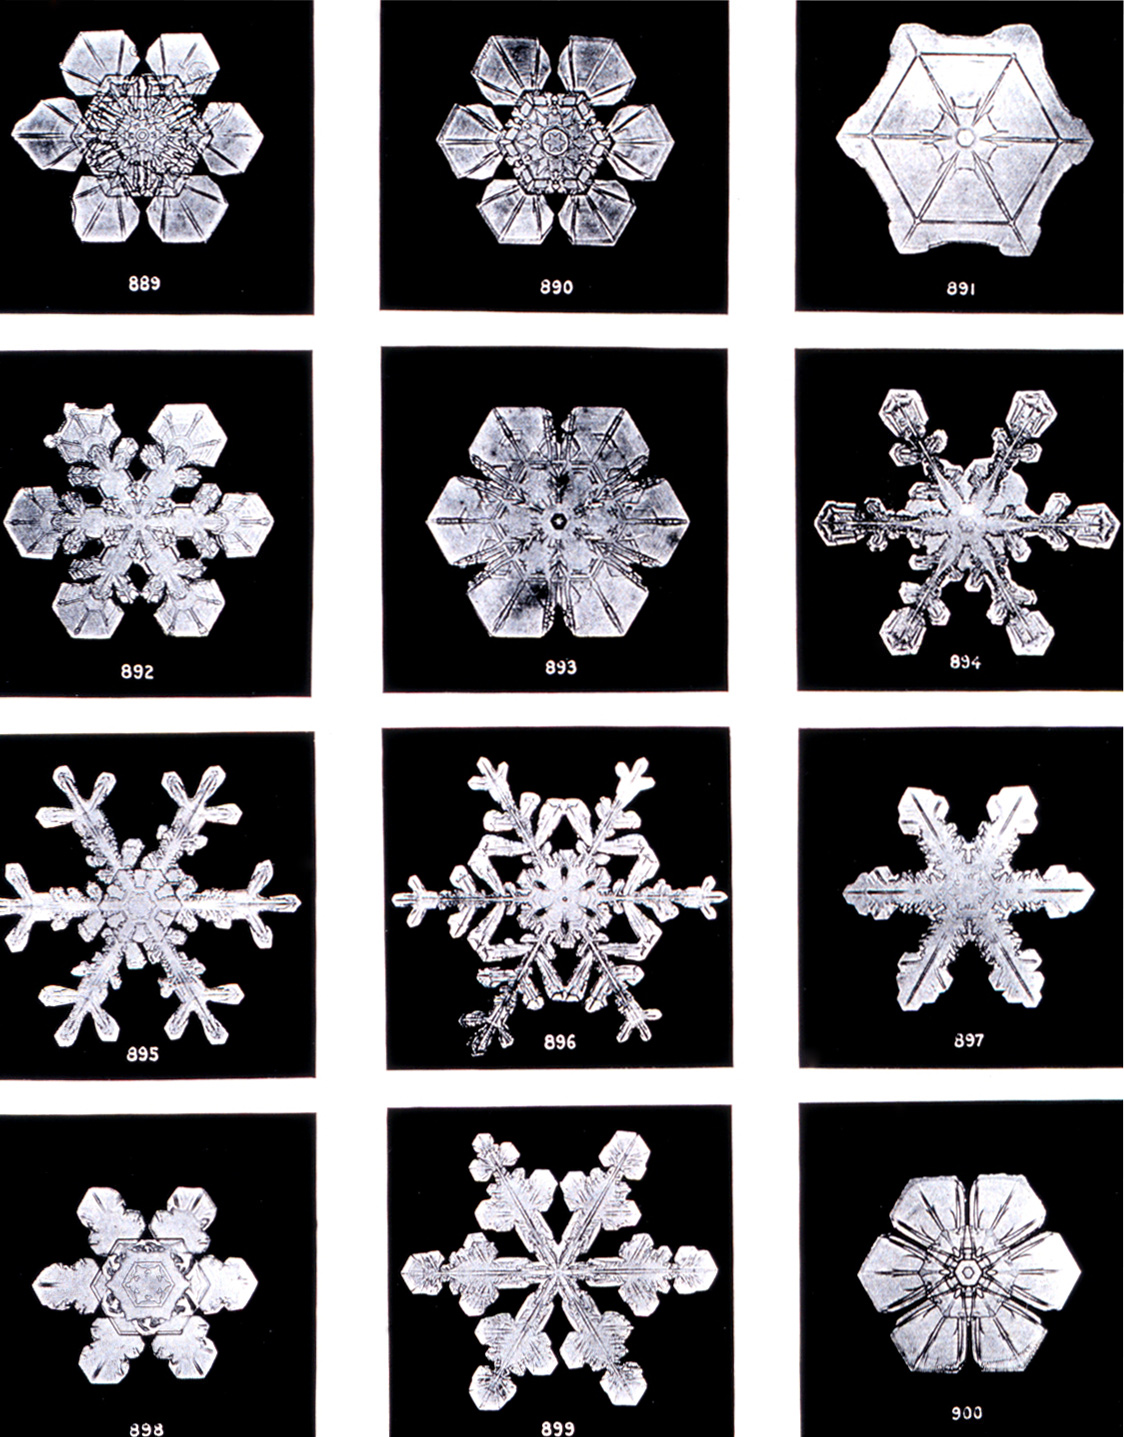
\includegraphics[width=0.36\linewidth]{images/book1/snowflakes.jpg}

{\small Des cristaux de neige photographiés par Wilson Bentley au début
des années 1900~: chacun a six branches.}
\end{omfigure}

\section{Exercices}


\begin{exercise}[$\star$]\label{exo:g11:polarity-and-cohesion:1}
Dans les liaisons \ce{H-Cl}, \ce{O-H} et \ce{C-O}, quel \omterm{def:g7:atoms-and-molecules:atom}{atome} porte la
\omterm{def:g11:polarity-and-cohesion:polar-bond}{charge partielle} $\delta^-$~? Utiliser le tableau des
\omterm{def:g11:polarity-and-cohesion:electronegativity}{électronégativités}.
\end{exercise}

\begin{exercise}[$\star$]\label{exo:g11:polarity-and-cohesion:2}
Parmi ces liaisons, lesquelles sont polarisées~: \ce{H-H}, \ce{C-H},
\ce{O-H}, \ce{N-H}, \ce{Cl-Cl}, \ce{C-Cl}~? Donner pour chacune la
différence d'\omterm{def:g11:polarity-and-cohesion:electronegativity}{électronégativité}.
\end{exercise}

\begin{exercise}[$\star$]\label{exo:g11:polarity-and-cohesion:3}
Quel est l'élément le plus électronégatif de chaque paire~: azote ou
phosphore~; oxygène ou soufre~; carbone ou azote~; sodium ou
magnésium~? Quelle tendance du tableau chaque paire illustre-t-elle~?
\end{exercise}

\begin{exercise}[$\star$]\label{exo:g11:polarity-and-cohesion:4}
Lesquelles des \omterm{def:g7:atoms-and-molecules:molecule}{molécules} \ce{CH4}, \ce{NH3}, \ce{H2O} et \ce{HCl}
peuvent-elles former des \omterm{def:g11:polarity-and-cohesion:hydrogen-bond}{liaisons hydrogène} entre elles~? Expliquer.
\end{exercise}

\begin{exercise}[$\star$]\label{exo:g11:polarity-and-cohesion:5}
Existe-t-il des attractions entre les \omterm{def:g11:polarity-and-cohesion:polar-molecule}{molécules apolaires} du méthane~?
Pourquoi le méthane est-il néanmoins un gaz à température ambiante~?
\end{exercise}

\begin{exercise}[$\star\star$]\label{exo:g11:polarity-and-cohesion:6}
Dire si chaque \omterm{def:g7:atoms-and-molecules:molecule}{molécule} est polaire~: le dichlorométhane \ce{CH2Cl2}
(tétraédrique), le tétrachlorométhane \ce{CCl4}, l'ammoniac \ce{NH3}, le
dioxyde de carbone \ce{CO2}, le trifluorure de bore \ce{BF3} (un
triangle plan avec le bore au centre).
\end{exercise}

\begin{exercise}[$\star\star$]\label{exo:g11:polarity-and-cohesion:7}
Dans le méthanol, \ce{CH3-OH}, quel \omterm{def:g7:atoms-and-molecules:atom}{atome} d'hydrogène peut être donné
dans une \omterm{def:g11:polarity-and-cohesion:hydrogen-bond}{liaison hydrogène}~? Quel \omterm{def:g7:atoms-and-molecules:atom}{atome} peut en recevoir une~? Les
\omterm{def:g7:atoms-and-molecules:molecule}{molécules} de méthanol et d'eau peuvent-elles former des \omterm{def:g11:polarity-and-cohesion:hydrogen-bond}{liaisons
hydrogène} entre elles~? En représenter une.
\end{exercise}

\begin{exercise}[$\star\star$]\label{exo:g11:polarity-and-cohesion:8}
Expliquer pourquoi les températures d'ébullition augmentent dans
l'ordre \ce{CH4} < \ce{SiH4} < \ce{GeH4}.
\end{exercise}

\begin{exercise}[$\star\star$]\label{exo:g11:polarity-and-cohesion:9}
Sur le graphique des températures d'ébullition des hydrures, quel
groupe ne présente aucune valeur anormale pour son premier composé~?
Pourquoi~?
\end{exercise}

\begin{exercise}[$\star\star$]\label{exo:g11:polarity-and-cohesion:10}
% ledger: en:H, en:Cl, en:Br, en:I, bp:HCl, bp:HBr, bp:HI
Les liaisons \ce{H-Cl}, \ce{H-Br}, \ce{H-I} sont de moins en moins
polarisées (les \omterm{def:g11:polarity-and-cohesion:electronegativity}{électronégativités} du chlore, du brome et de l'iode
valent 3.16, 2.96 et 2.66), et pourtant les températures d'ébullition
augmentent~: \qty{-85}{\celsius}, \qty{-66}{\celsius},
\qty{-35}{\celsius}. Quelle interaction l'emporte, et pourquoi~?
\end{exercise}

\begin{exercise}[$\star\star$]\label{exo:g11:polarity-and-cohesion:11}
À température ambiante, le dichlore est un gaz et le diiode un solide,
bien que tous deux soient formés de \omterm{def:g11:polarity-and-cohesion:polar-molecule}{molécules apolaires} \ce{X2}.
Expliquer.
\end{exercise}

\begin{exercise}[$\star\star\star$]\label{exo:g11:polarity-and-cohesion:12}
% ledger: bp:C2H5OH, bp:CH3OCH3, bp:C3H8
L'éthanol \ce{CH3-CH2-OH}, le méthoxyméthane \ce{CH3-O-CH3} et le propane
\ce{CH3-CH2-CH3} ont presque la même \omterm{def:g10:the-mole:molar-mass}{masse molaire}. Ils bouillent à
\qty{78}{\celsius}, \qty{-25}{\celsius} et \qty{-42}{\celsius}. Lesquels
sont polaires~? Lesquels forment des \omterm{def:g11:polarity-and-cohesion:hydrogen-bond}{liaisons hydrogène} entre leurs
propres \omterm{def:g7:atoms-and-molecules:molecule}{molécules}~? Expliquer l'ordre.
\end{exercise}

\begin{exercise}[$\star\star\star$]\label{exo:g11:polarity-and-cohesion:13}
Dans la glace, chaque \omterm{def:g7:atoms-and-molecules:molecule}{molécule} d'eau est liée par \omterm{def:g11:polarity-and-cohesion:hydrogen-bond}{liaisons hydrogène} à
quatre voisines, en un réseau ouvert~; dans l'eau liquide, le réseau se
rompt sans cesse et s'effondre en partie. Expliquer pourquoi la glace
flotte sur l'eau. Pourquoi est-ce important pour les poissons d'un lac
gelé~?
\end{exercise}

\begin{exercise}[$\star\star\star$]\label{exo:g11:polarity-and-cohesion:14}
Classer par température de fusion croissante, en justifiant par les
attractions entre les particules~: le chlorure de potassium \ce{KCl}, la
glace \ce{H2O}, le méthane solide \ce{CH4}.
\end{exercise}

\begin{exercise}[$\star\star\star$]\label{exo:g11:polarity-and-cohesion:15}
% ledger: en:F, en:O, bp:HF, bp:H2O
Le fluor est plus électronégatif que l'oxygène~: une liaison \ce{H-F} est
donc plus polarisée qu'une liaison \ce{O-H}. Pourtant, l'eau bout à
\qty{100}{\celsius} et le fluorure d'hydrogène à \qty{20}{\celsius}.
Compter les \omterm{def:g7:atoms-and-molecules:atom}{atomes} d'hydrogène que chaque \omterm{def:g7:atoms-and-molecules:molecule}{molécule} peut donner et les
\omterm{def:g10:lewis-and-shape:lone-pair}{doublets non liants} avec lesquels elle peut en recevoir, et expliquer.
\end{exercise}

\section{Problème~: pourquoi l'eau bout-elle à \texorpdfstring{\qty{100}{\celsius}}{100 degrés Celsius}~?}

\begin{problem}[{Problème du week-end --- sans liaisons hydrogène, à quelle
température l'eau bouillirait-elle~?}]
\label{pb:g11:polarity-and-cohesion:1}
% ledger: en:H, en:O, en:S, en:Se, bp:H2O, bp:H2S, bp:H2Se, bp:CH4, bp:SiH4, bp:GeH4, bp:HCl, bp:HBr, bp:HF, bp:NH3, bp:PH3, bp:AsH3
L'oxygène, le soufre et le sélénium sont dans le même groupe du tableau,
et tous trois forment un composé avec l'hydrogène~: \ce{H2O}, \ce{H2S},
\ce{H2Se}. Dans chaque groupe d'hydrures, les températures d'ébullition
augmentent en général avec la taille de la \omterm{def:g7:atoms-and-molecules:molecule}{molécule}. L'eau fait
exception. De combien~?

\medskip
\noindent\textbf{Partie I --- Trois \omterm{def:g7:atoms-and-molecules:molecule}{molécules}.}
\begin{enumerate}
  \item Établir les \omterm{def:g10:lewis-and-shape:lewis-structure}{schémas de Lewis} de \ce{H2O}, \ce{H2S} et \ce{H2Se}.
        Pourquoi se ressemblent-ils~?
  \item Calculer leurs \omterm{def:g10:the-mole:molar-mass}{masses molaires}.
  \item Calculer les différences d'\omterm{def:g11:polarity-and-cohesion:electronegativity}{électronégativité} des liaisons
        \ce{O-H}, \ce{S-H} et \ce{Se-H} (oxygène 3.44, soufre 2.58,
        sélénium 2.55, hydrogène 2.20). Quelles liaisons sont nettement
        polarisées~?
  \item Quelle est la géométrie des trois \omterm{def:g7:atoms-and-molecules:molecule}{molécules}~? Sont-elles
        polaires~?
  \item Compter les \omterm{def:g9:inside-the-atom:nucleus}{électrons} de chaque \omterm{def:g7:atoms-and-molecules:molecule}{molécule}. Laquelle a les
        \omterm{def:g11:polarity-and-cohesion:van-der-waals}{interactions de van der Waals} les plus fortes~?
\end{enumerate}

\medskip
\noindent\textbf{Partie II --- Les \omterm{def:g11:polarity-and-cohesion:hydrogen-bond}{liaisons hydrogène}.}
\begin{enumerate}[resume]
  \item Lequel des trois composés forme des \omterm{def:g11:polarity-and-cohesion:hydrogen-bond}{liaisons hydrogène} entre ses
        \omterm{def:g7:atoms-and-molecules:molecule}{molécules}~? Pourquoi pas les autres~?
  \item À combien de \omterm{def:g11:polarity-and-cohesion:hydrogen-bond}{liaisons hydrogène} une \omterm{def:g7:atoms-and-molecules:molecule}{molécule} d'eau peut-elle
        participer au plus~? Les représenter.
  \item Quelles interactions retiennent les \omterm{def:g7:atoms-and-molecules:molecule}{molécules} de sulfure
        d'hydrogène entre elles dans le liquide~?
\end{enumerate}

\medskip
\noindent\textbf{Partie III --- La tendance.}
\begin{enumerate}[resume]
  \item Le sulfure d'hydrogène bout à \qty{212.9}{K} et le séléniure
        d'hydrogène à \qty{-41.3}{\celsius}. Exprimer la
        première en degrés Celsius ($\theta = T - 273.15$).
  \item De combien la température d'ébullition augmente-t-elle de la
        \omterm{def:g9:periodic-table-first-look:period}{période} 3 (\ce{H2S}) à la \omterm{def:g9:periodic-table-first-look:period}{période} 4 (\ce{H2Se})~?
  \item Pourquoi augmente-t-elle~?
  \item En supposant la même augmentation de la \omterm{def:g9:periodic-table-first-look:period}{période} 2 à la
        \omterm{def:g9:periodic-table-first-look:period}{période} 3, à quelle température bouillirait une eau «~normale~»
        \ce{H2O}~?
  \item Tester la méthode sur le \omterm{def:g9:periodic-table-first-look:period}{groupe} 14~: \ce{SiH4} bout à
        \qty{-112}{\celsius} et \ce{GeH4} à \qty{-88.1}{\celsius}.
        Prévoir la température d'ébullition de \ce{CH4} et la comparer à
        la valeur réelle, \qty{-162}{\celsius}. L'extrapolation est-elle
        exacte~?
  \item Faire de même pour le \omterm{def:g9:periodic-table-first-look:period}{groupe} 17 (\ce{HCl} \qty{-85.1}{\celsius},
        \ce{HBr} \qty{-66.4}{\celsius}) et comparer avec \ce{HF},
        \qty{19.6}{\celsius}.
\end{enumerate}

\medskip
\noindent\textbf{Partie IV --- L'écart.}
\begin{enumerate}[resume]
  \item L'eau bout réellement à \qty{100}{\celsius}. Quel est l'écart
        entre la valeur réelle et la valeur extrapolée~?
  \item Même question pour l'ammoniac, à l'aide de \ce{PH3}
        \qty{-87.8}{\celsius} et \ce{AsH3} \qty{-62.5}{\celsius}~;
        l'ammoniac bout réellement à \qty{-33.4}{\celsius}.
  \item Classer l'eau, le fluorure d'hydrogène et l'ammoniac selon la
        taille de leur écart, et expliquer ce classement en comptant les
        \omterm{def:g11:polarity-and-cohesion:hydrogen-bond}{liaisons hydrogène}.
  \item Sans \omterm{def:g11:polarity-and-cohesion:hydrogen-bond}{liaisons hydrogène}, l'eau serait-elle solide, liquide ou
        gazeuse à température ambiante~? Que cela signifierait-il pour la
        Terre~?
  \item Pourquoi la réponse à la question 12 n'est-elle qu'une
        estimation~?
  \item Donner la réponse finale~: à quelle température environ l'eau
        bouillirait-elle sans \omterm{def:g11:polarity-and-cohesion:hydrogen-bond}{liaisons hydrogène}~?
\end{enumerate}
\end{problem}
